\chapter{Expériences numériques}\label{Chap::Resultat}
	\minitoc

Après avoir étudié les propriétés observationnelles des amas globulaires et des galaxies, nous avons mis en évidence un certain nombre
de résultats analytiques sur diverses sphères isothermes. Nous allons maintenant entreprendre des simulations numériques visant
à illustrer ces divers résultats et constats.

Les expériences que nous allons mener consistent à étudier la dynamique d'un système auto-gravitant (\textsc{sag}) placé
dans un bain thermique. Ces conditions respectent celles du problème détaillé dans la section~\ref{Sec::ToyModel}.

Afin de préserver l'intégrité de nos différents systèmes, nous avons imposé aux particules du bain et du \textsc{sag} d'avoir la
même masse.

\section{Description des conditions initiales}

	Nous avons utilisé principalement deux types de bain:
	\begin{description}

		\item[Un thermostat:] ce type de bain est construit de sorte à se comporter comme un
			thermostat. Il s'agit d'un cube périodique, dans lequel les particules massives sont
			réparties spatialement selon une distribution uniforme. La température est fixée par la
			distribution gaussienne attribuée aux vitesses. Un thermostat maintient une
			température sans être affecté par le système avec lequel il est en contact.
			Nous faisons donc en sorte que les particules de ce bain puissent influer sur les
			particules du \textsc{sag} sans que celles-ci n'affectent celles du bain en utilisant
			une option de Gadget.

		\item[Un réservoir thermique:] il s'agit d'un système composé de particules massives réparties
			uniformément dans un cube périodique et dont la température est aussi fixée par une
			distribution gaussienne des vitesses. Contrairement au thermostat, les particules du
			réservoir ressentent l'interaction gravitationnelle des particules du \textsc{sag}.

	\end{description}

	Les paramètres du réservoir et du thermostat sont les suivants:
	\begin{itemize}
		\item le nombre de particules $N_b$;
		\item la température $T$;
		\item le côté du cube $R_c$.
	\end{itemize}
	Ces paramètres sont indépendants et constituent une partie de l'espace des paramètres de nos
	simulations. La stabilité du réservoir thermique va dépendre des valeurs de ces paramètres, notamment à
	travers le critère de Jeans (voir la section~\ref{Chap::Instabilite::Sec::Jeans}).

	\begin{figure}[hbt]
		\begin{center}
			\begin{tikzpicture}
				\draw[pattern=north east lines] (-2, 2) rectangle (2, -2);
				% \draw (-2, 2) grid[step=0.2] (2, -2);

				\draw[fill=red!70,opacity=0.5] (0, 0) circle (0.5);
				% \node[fill=white,opacity=0.8] at (0, 0) {\textsc{sag}};

				% \node at (-2, 2) [below right, fill=white,opacity=0.8] {Bain};
				\node at (-2, -2) [above right, fill=white,opacity=0.8] {$T$, $N$};
				\draw[<->] (-2, -2.2) -- (2, -2.2);
				\node at (0, -2.2) [below] {$R_c$};

				\draw[pattern=north east lines] (2.5, 1.8) rectangle (3, 1.5) node at (3.1, 1.65) [right] {Bain};
				\draw[fill=red!70,opacity=0.5] (2.5, 1.3) rectangle (3, 1.0) node at (3.1, 1.15) [right,opacity=1.0] {\textsc{sag}};
			\end{tikzpicture}
			\caption{Condition initiale des simulations.\label{Fig::CI::Repr}}
		\end{center}
	\end{figure}

	L'effet d'un thermostat sur le \textsc{sag} ne peut a priori se faire qu'aux travers des collisions~\footnote{par collisions, nous entendons
	des interactions à deux corps.}, les particules du thermostat ne pouvant être capturées par le \textsc{sag}. L'effet correspondant ne peut
	alors apparaître que sur des temps grands devant le temps dynamique du \textsc{sag}. Un réservoir thermique sera a priori plus efficace, les
	interactions gravitationnelles pouvant amener une partie des particules du réservoir à être capturées par le \textsc{sag}, ou réciproquement.
	Des effets peuvent donc apparaître plus rapidement.

	Nous avons utilisé deux types de \textsc{sag}:
	\begin{itemize}
		\item un modèle de King, dont les paramètres (définis dans le chapitre~\ref{King::Chapitre}) sont $W_0$, $\sigma$, $r_c$ et le nombre
			de particules $N_K$;
		\item une sphère de Hénon, de rayon initial $R$, de masse $M$, de viriel initial $\gamma$ et contenant $N_H$ particules.
	\end{itemize}

	La figure~\ref{Fig::CI::Repr} représente la répartition initiale du bain et du \textsc{sag}. À ce moment, des particules du bain se trouvent déjà dans le \textsc{sag}.

\section{Étude préliminaire}

	Une première série de simulations a consisté à placer un modèle de King, de paramètre $W_0 = 5,2$, $\sigma_c = 2,9\
	\mathrm{km}.\mathrm{s}^{-1}$ et $r_c = 3,5\ \mathrm{pc}$, dans un thermostat. Les paramètres de chaque simulation étaient la température du
	bain, la taille de la boîte et le nombre de particules utilisées dans chacun des deux systèmes. La taille de la boîte nous permet de jouer sur
	la densité du bain. La température était calculée pour être un multiple $k$ de la température moyenne de la sphère de King initiale. Nous
	avons fait varier $k$ dans l'intervalle $10^{-3}$ à $10^5$. Chaque configuration initiale a évolué sur des périodes de temps allant de $10T_d$
	à $120T_d$, où $T_d$ est le temps dynamique de la sphère de King initiale (voir le chapitre~\ref{Chap::TempsCarac}). De plus, nous avons
	ajusté le paramètre de lissage de la force $\epsilon$ de sorte que le \textsc{sag} utilisé ne soit pas affecté par les effets de relaxations à deux
	corps. Ni la densité du \textsc{sag} ni les autres paramètres n'ont jamais montré de véritable évolution lors de ces simulations.
	% Ces résultats semblent indiquer que nous avons correctement ajusté le paramètre $\epsilon$.

	% PLACER QUELQUES GRAPHES.

	Face à ce constat, nous avons augmenté la sensibilité de nos simulations en remplaçant le thermostat par un réservoir thermique et la
	sphère de King par une sphère de Hénon.

\section{Seconde étude}\label{Sec::2ndStudy}

	Une seconde série de simulations est construite en utilisant une sphère Hénon de rayon $R=2$, de masse $M=1$, de viriel $\gamma=-0,5$,
	contenant $N_H = 30000$ particules et placée dans un réservoir thermique. Nous utiliserons ici le même système d'unité que dans le
	chapitre~\ref{Chap::VlasovGadget}, dans lequel le temps dynamique du \textsc{sag} est $T_d^{t=0} = 2\pi$. De la même façon que lors de l'étude
	précédente, nous allons utiliser les caractéristiques du réservoir comme paramètres des simulations: le nombre de particules $N_b$, la taille
	du cube $R_c$ et sa température $\sigma_c$. Globalement l'évolution dynamique de ce système montre toujours deux phases successives.

	Dans un premier temps, la sphère de Hénon s'effondre et forme, comme attendu pour $\gamma=-0,5$ (\citet{roy}, \citet{Joyceetal}), une
	structure cœur-halo de pente $\alpha\simeq-4$ (\textsc{ch4}) à l'équilibre ($\gamma=-1$). La durée de cette phase initiale est de l'ordre de
	quelques temps dynamiques de la sphère de Hénon initiale. Cette phase d'effondrement n'est pratiquement pas affectée par les paramètres du
	réservoir. L'intersection des deux systèmes (bain et \textsc{sag}) n'étant pas vide, le nombre de particules du bain contenu dans le
	\textsc{sag} est variable, ce qui explique la légère variation observée des paramètres post-effondrement. La
	figure~\ref{Fig::Simu::EvoParamPostCollapse} indique, après l'effondrement, les valeurs des différents rayons, axes d'inertie, viriel,
	température et anisotropie en fonction des paramètres du réservoir thermique pour une partie représentative de nos simulation. Ces valeurs
	sont calculées en faisant la moyenne de chaque paramètre dans l'intervalle $[1T_d^{t=0}; 1,5T_d^{t=0}]$. Cette phase d'effondrement est la
	traduction de l'instabilité de Jeans.
	\begin{figure}[htbp]
		\centering \rotatebox{90}{%
			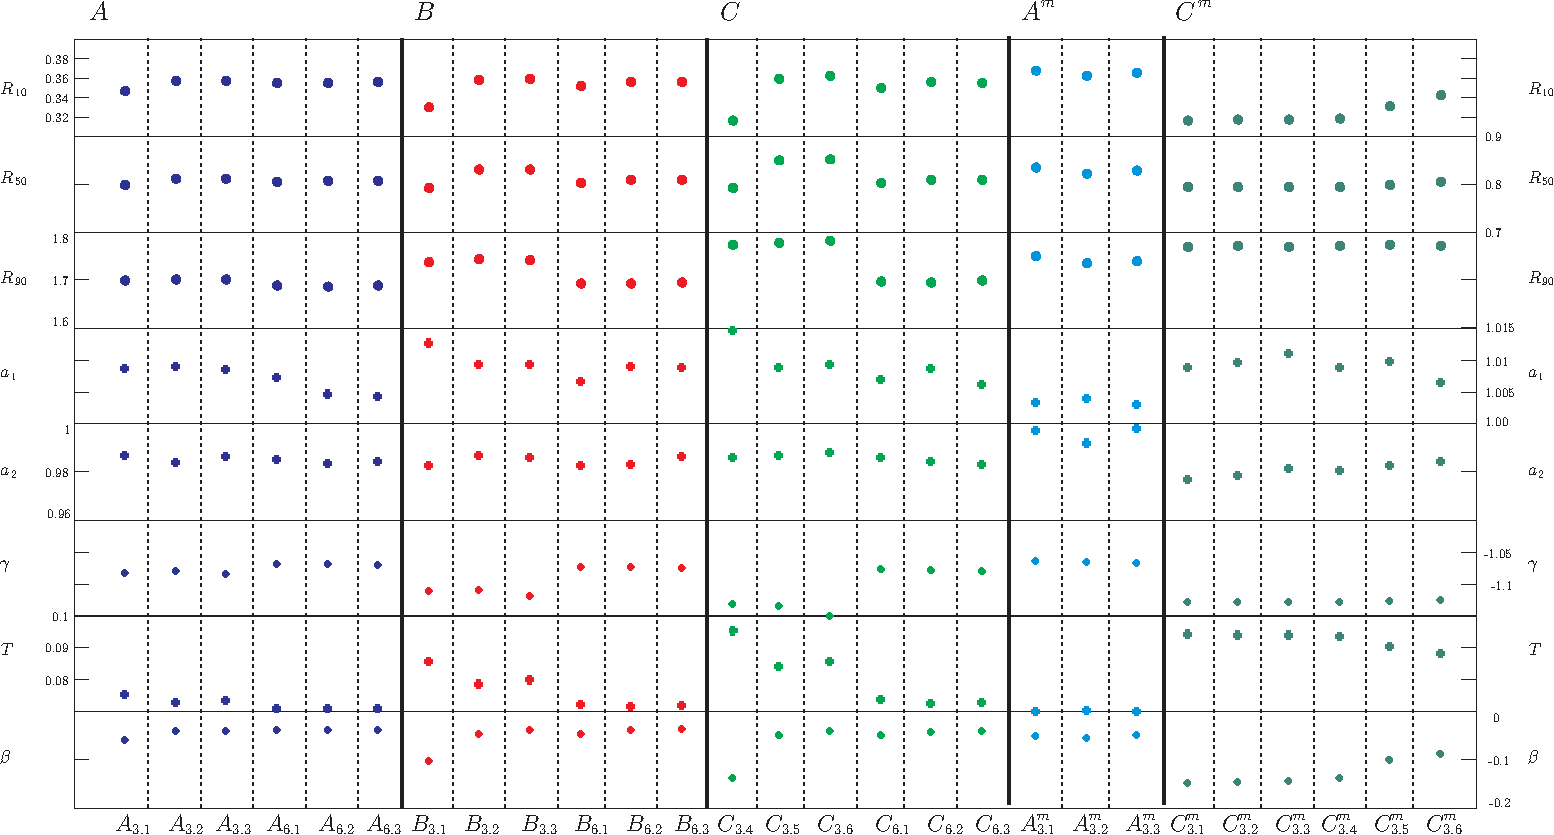
\includegraphics[scale=0.8]{graphe/post-collapse.pdf}%
		}
		\caption{Valeur des différentes observables après l'effondrement en fonction des paramètres du bain thermique.\label{Fig::Simu::EvoParamPostCollapse}}
	\end{figure}

	L'évolution dynamique post-effondrement de cette structure de type \textsc{ch4} est alors influencée par le bain. Cette influence est modulée
	par les paramètres du réservoir thermique. Nous avons effectué plus de 300 simulations dans l'espace des paramètres, la
	table~\ref{Tab::SimuZoomRes} résume l'évolution dynamique d'une partie représentative de ces simulations. Cette évolution s'étend jusqu'à un
	temps correspondant à $15.9 T_d^{t=0}$.
	Les observables étudiées sont celles définies dans le chapitre~\ref{Chap::Simu::Analysis}, nous avons regroupé leur évolution dynamique en
	différentes classes associées aux symboles suivants:
	\begin{table}[htbp]
		% \begin{tabular}{|m{1.5cm}|m{1cm}|m{2cm}|m{2cm}|m{2.5cm}|m{2.0cm}|m{2cm}|}
	% Vérifier la pente du halo et ajouter celle du centre
	\centering
		\begin{tabular}{|c|c|c|c|c|c|c|c|c|c|}
			\hline $N$ & $R_c$ & $\sigma_c$ & $R_{10}$, $R_{50}$, $R_{90}$ & $a_1$, $a_2$ & $\beta$ & $\rho$ & $T$ & $\gamma$ & nom \tabularnewline
			\hline
			\hline \multirow{6}{*}{$1\ 10^5$} & \multirow{3}{*}{$33.3$}
					% & $10^{-3}$ & Accrétion & Triaxialisation du \textsc{sag} & tend vers $-0,5$ & Évolution de la pente du halo \tabularnewline \cline{3-7}
					% & $10^{-3}$ & Accrétion & \begin{tikzpicture}\node[draw,ellipse] at (0,0) {}; \end{tikzpicture}Triaxialisation du \textsc{sag} & tend vers $-0,5$ & Évolution de la pente du halo \tabularnewline \cline{3-7}
					& $10^{-3}$ & \accretionmoyen{} & $\diamondsuit$ & ${}_{0.15}\nearrow^{0.43}$ & $\alpha\searrow$ & $\nearrow$ & $\searrow$ & $A_{3,1}$ \tabularnewline \cline{3-10}
					& & $10^{-1}$ & \accretionpeu{} & $\emptyset$ & ${}^{0.02}\searrow_{-0.1}$ & $\emptyset$ & $\nearrow$ & $\emptyset$ & $A_{3,2}$  \tabularnewline \cline{3-10}
					& & $2\ 10^{-1}$ & \accretionpeu{} & $\emptyset$ & ${}^{0.02}\searrow_{-0.11}$ & $\emptyset$ & $\nearrow$ & $\emptyset$ & $A_{3,3}$  \tabularnewline \cline{2-10}
				& \multirow{3}{*}{$66.6$}
					& $10^{-3}$ & \accretionpeu{} & $\emptyset$ & ${}^{0.08}\searrow_{0.03}$ & $\emptyset$ & $\nearrow$ & $\searrow$ & $A_{6,1}$  \tabularnewline \cline{3-10}
					& & $10^{-1}$ & \accretionpeu{} & $\emptyset$ & ${}^{0.06}\searrow_{-0.11}$ & $\emptyset$ & $\nearrow$ & $\emptyset$ & $A_{6,2}$  \tabularnewline \cline{3-10}
					& & $2\ 10^{-1}$ & \accretionpeu{} & $\emptyset$ & ${}^{0.06}\searrow_{-0.12}$ & $\emptyset$ & $\nearrow$ & $\emptyset$ & $A_{6,3}$  \tabularnewline \cline{2-10}
			\hline
			\hline $2\ 10^5$ & $66.6$ & $10^{-3}$ & \accretionpeu{} & $\emptyset$ & ${}_{0.1}\nearrow^{0.17}$ & $\alpha\searrow$ & $\nearrow$ & $\emptyset$ & $A_{6,1}^m$  \\
			\hline
			\hline $4\ 10^5$ & $66.6$ & $10^{-3}$ & \accretionpeu{} & $\emptyset$ & ${}_{0.1}\nearrow^{0.23}$ & $\alpha\searrow$ & $\nearrow$ & $\emptyset$ & $A_{6,2}^m$  \\
			\hline
			\hline $1\ 10^6$ & $66.6$ & $10^{-3}$ & \accretionpeu{} & $\emptyset$ & ${}_{0.12}\nearrow^{0.27}$ & $\alpha\searrow$ & $\nearrow$ & $\emptyset$ & $A_{6,3}^m$  \\
			\hline
			\hline \multirow{6}{*}{$3.25\ 10^5$} & \multirow{3}{*}{$33.3$}
					& $10^{-3}$ & \accretionlot{} & $\spadesuit$ & ${}^{0.36}\searrow_{0.33}$ & $\alpha\searrow$ & $\nearrow$ & $\searrow$ & $B_{3,1}$  \tabularnewline \cline{3-10}
					& & $10^{-1}$ & \accretionpeu{} & $\emptyset$ & ${}^{0.05}\searrow_{0.0}$ & $\emptyset$ & $\nearrow$ & $\searrow$ & $B_{3,2}$  \tabularnewline \cline{3-10}
					& & $2\ 10^{-1}$ & \accretionpeu{} & $\emptyset$ & ${}^{0.03}\searrow_{-0.05}$ & $\emptyset$ & $\nearrow$ & $\emptyset$ & $B_{3,3}$  \tabularnewline \cline{2-10}
				& \multirow{3}{*}{$66.6$}
					& $10^{-3}$ & \accretionpeu{} & $\emptyset$ & ${}_{0.11}\nearrow^{0.42}$ & $\alpha\searrow$ & $\nearrow$ & $\searrow$ & $B_{6,1}$  \tabularnewline \cline{3-10}
					& & $10^{-1}$ & \accretionpeu{} & $\emptyset$ & ${}^{0.06}\searrow_{-0.1}$ & $\emptyset$ & $\nearrow$ & $\emptyset$ & $B_{6,2}$  \tabularnewline \cline{3-10}
					& & $2\ 10^{-1}$ & \accretionpeu{} & $\emptyset$ & ${}^{0.06}\searrow_{-0.1}$ & $\emptyset$ & $\nearrow$ & $\emptyset$ & $B_{6,3}$  \tabularnewline \cline{2-10}
			\hline
			\hline \multirow{6}{*}{$5.5\ 10^5$} & \multirow{3}{*}{$33.3$}
					& $10^{-3}$ & \accretionlot{} & $\spadesuit$ & ${}_{0.5}\nearrow^{0.37}$ & $\alpha\searrow$ & $\nearrow$ & $\searrow$ & $C_{3,4}$  \tabularnewline \cline{3-10}
					& & $10^{-1}$ & \accretionlot{} & $\emptyset$ & ${}^{0.07}\searrow_{0.03}$ & $\emptyset$ & $\nearrow$ & $\searrow$ & $C_{3,5}$  \tabularnewline \cline{3-10}
					& & $2\ 10^{-1}$ & \accretionpeu{} & $\emptyset$ & ${}^{0.04}\searrow_{-0.01}$ & $\emptyset$ & $\nearrow$ & $\searrow$ & $C_{3,6}$  \tabularnewline \cline{2-10}
				& \multirow{3}{*}{$66.6$}
					& $10^{-3}$ & \accretionmoyen{} & $\spadesuit$ & ${}_{0.15}\nearrow^{0.67}$ & $\alpha\searrow$ & $\nearrow$ & $\searrow$ & $C_{6,1}$  \tabularnewline \cline{3-10}
					& & $10^{-1}$ & \accretionpeu{} & $\emptyset$ & ${}^{0.06}\searrow_{-0.07}$ & $\emptyset$ & $\nearrow$ & $\emptyset$ & $C_{6,2}$  \tabularnewline \cline{3-10}
					& & $2\ 10^{-1}$ & \accretionpeu{} & $\emptyset$ & ${}^{0.05}\searrow_{-0.1}$ & $\emptyset$ & $\nearrow$ & $\emptyset$ & $C_{6,3}$  \tabularnewline \cline{2-10}
			\hline
			\hline \multirow{6}{*}{$1856250$} & \multirow{6}{*}{$50$}
					& $1,25\ 10^{-4}$ & \accretionlot{} & $\spadesuit$ & ${}^{0.5}\searrow_{0.13}$ & $\alpha\searrow$ & $\nearrow$ & $\searrow$ & $C_{3,1}^m$  \tabularnewline \cline{3-10}
					& & $2,5\ 10^{-4}$ & \accretionlot{} & $\spadesuit$ & ${}^{0.5}\searrow_{0.28}$ & $\alpha\searrow$ & $\nearrow$ & $\searrow$ & $C_{3,2}^m$  \tabularnewline \cline{3-10}
					& & $5\ 10^{-4}$ & \accretionlot{} & $\spadesuit$ & ${}^{0.5}\searrow_{0.22}$ & $\alpha\searrow$ & $\nearrow$ & $\searrow$ & $C_{3,3}^m$  \tabularnewline \cline{3-10}
					& & $10^{-3}$ & \accretionlot{} & $\spadesuit$ & ${}^{0.5}\searrow_{0.24}$ & $\alpha\searrow$ & $\nearrow$ & $\searrow$ & $C_{3,4}^m$  \tabularnewline \cline{3-10}
					& & $10^{-1}$ & \accretionlot{} & $\emptyset$ & ${\scriptstyle 0.36}\to{\scriptstyle 0.36}$ & $\alpha\searrow$ & $\nearrow$ & $\searrow$ & $C_{3,5}^m$  \tabularnewline \cline{3-10}
					& & $2\ 10^{-1}$ & \accretionlot{} & $\emptyset$ & ${}_{0.3}\nearrow^{0.36}$ & $\emptyset$ & $\nearrow$ & $\searrow$ & $C_{3,6}^m$  \tabularnewline \cline{2-10}
			\hline
		\end{tabular}
	\caption{Résultats des simulations combinant un Hénon et un réservoir thermique.\label{Tab::SimuZoomRes}}
\end{table}



	\begin{itemize}

		\item Les variations des observables $R_{10}$, $R_{50}$ et $R_{90}$ peuvent être regroupées en 3 classes:
			\begin{itemize}

				\item[\accretionpeu{}] indique que $R_{10}$ et $R_{50}$ diminuent (de $5\%$ à $40\%$); le cœur du \textsc{sag} se
					contracte alors que $R_{90}$ varie de $-15\%$ à $60\%$.

				\item[\accretionmoyen{}] indique une accrétion modérée du bain par le \textsc{sag}. Le rayon $R_{10}$ continue
					à décroitre (de l'ordre de $20\%$) alors que $R_{50}$ et $R_{90}$ croissent. La variation de $R_{50}$ peut
					atteindre $30\%$ tandis que $R_{90}$ peut aller jusqu'à doubler.

				\item[\accretionlot{}] indique une forte accrétion du bain par le \textsc{sag}. Tous les rayons caractéristiques sont
					au minimum doublés sur l'évolution dynamique du système.
			\end{itemize}

		\item Les variations des rapports d'axes mettent en évidence 3 évolutions distinctes:
			\begin{itemize}

				\item[$\spadesuit$] indique l'apparition d'une déformation du système au cours de laquelle $a_1 \simeq 1$ et $a_2 \to 0,4$.

				\item[$\emptyset$] indique que le système conserve sa forme sphérique.

				\item[$\diamondsuit$] est un cas particulier qui sera détaillé un peu plus loin.

			\end{itemize}
	\end{itemize}

	Une première analyse est alors possible: % nous apprend:
	\begin{enumerate}

		\item les simulations auxquelles sont associées les symboles \accretionlot{} et $\spadesuit$ présentent également une évolution
			particulière de l'anisotropie. Ce paramètre passe par un minimum au moment où le \textsc{sag} se déforme. Ce type d'évolution
			peut-être interprété dans le contexte de l'instabilité d'orbite radiale.

		\item les simulations \accretionmoyen{} entrent dans une catégorie intermédiaire suggérant que les caractéristiques du bain, comme sa
			densité ou sa température, sont des paramètres importants dans le déclenchement de l'instabilité d'orbite radiale.

		\item les simulations \accretionpeu{} forment la dernière catégorie. La concentration du cœur présente dans ces simulations peut avoir
			une origine thermodynamique issue de la présence du Halo ou bien être la manifestation des effets de relaxation à 2 corps.
			L'étude faîte dans la section suivante tentera de répondre à cette question.
			% Ces simulations seront étudiées plus en détails dans la prochaine
			% section.

		\item la simulation caractérisée par le symbole $\diamondsuit$ est un cas limite où les résultats semblent affectés par les conditions
			périodiques.
			%sont des simulations très touchées par les conditions périodiques.
			Ces simulations vont avoir tendance à former des barres alignées sur les coins de la boîte. La
			figure~\ref{Fig::Density::Comp::Periodic} compare deux simulations, l'une subissant les effets de la boîte périodique, l'autre
			ne les subissant pas.
			\begin{figure}[hbtp]
				\begin{minipage}{0.49\linewidth}
					\centering 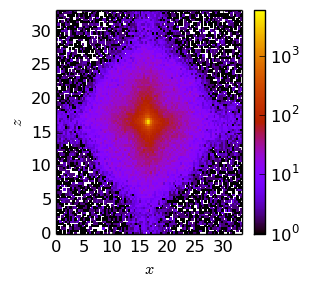
\includegraphics{{graphe/Periodique_Plot/N-100000.0_Rc-33.3333333333_sc-0.001_Soft-0.001}.png}
				\end{minipage}\hfill
				\begin{minipage}{0.50\linewidth}
					\centering 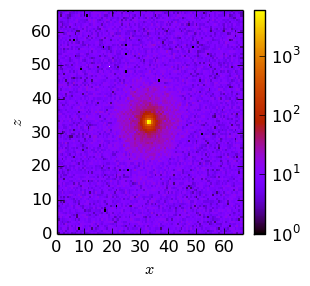
\includegraphics{{graphe/Periodique_Plot/N-100000.0_Rc-66.6666666666_sc-0.001_Soft-0.001}.png}
				\end{minipage}
				\caption{À gauche une simulation ($A_{3,1}$) sous l'influence des conditions périodiques, à droite une simulation ($A_{6,1}$) correcte.\label{Fig::Density::Comp::Periodic}}
			\end{figure}

	\end{enumerate}

	Pour rendre compte correctement de l'évolution dynamique, nous avons besoin d'une unité de temps capable de rendre compte de cette évolution.
	Les deux unités arrivant directement à l'esprit sont le temps dynamique et le temps de relaxations à deux corps (voir
	chapitre~\ref{Chap::TempsCarac}). Nous rappelons que le temps dynamique $T_d$ s'écrit:
	\begin{align*}
		T_d = \pi \sqrt{\dfrac{R^3}{2m\(R\)G}}
	\end{align*}
	et que le temps de relaxation à deux corps $T_\mathrm{rel}$ s'écrit (voir le chapitre~\ref{Chap::TempsCarac}):
	\begin{align*}
		T_\mathrm{rel} = \dfrac{Nm\(R\)}{4\pi^2R^3\rho\(R\)\ln\frac{R}{p_\mathrm{min}}} T_d
	\end{align*}
	avec $R$ un rayon caractéristique de l'objet, $m\(R\)$ la masse contenue dans le rayon $R$ et $\rho\(R\)$ la densité à ce même rayon. Quel rayon utiliser?
	Comme nous le verrons dans la section suivante, $R_{90}$ est très sensible à l'environnement, surtout pour les simulations de types
	(\accretionlot{}, $\spadesuit$). $R_{10}$ est plus intéressant mais ne rend compte que de l'évolution du cœur du système. $R_{50}$ semble
	ainsi le meilleur choix. Dans la suite, et sauf mention contraire, nous utiliserons le temps dynamique $T_d^{50\%}$ et le temps de relaxation
	à deux corps $T_\mathrm{rel}^{50\%}$ calculés avec $R_{50}$. Pour $p_\mathrm{min}$,
	nous prendrons la plus petite longueur caractéristique de nos simulation: le paramètre de lissage de la force
	$\epsilon$.

	% Le soucis avec ce temps caractéristique, c'est qu'il a des variations relativement importantes. Lorsque nous traçons nos observable en
	% fonction de $t_i' = \frac{t_i}{T_d^i}$, ces variations se traduisent par des \og{}retours en arrière\fg.
	
	Une estimation directe du temps de la simulation en unités de temps dynamique consisterait à utiliser une relation de la forme $t_i' =
	\frac{t_i}{T_d^i}$. Cependant les fluctuations de $T_d^i$ pourraient conduire à des \og{}retour en arrière\fg.
	Pour éviter cet effet, nous allons calculer une nouvelle échelle de temps comme suit:
	\begin{align*}
		t_i' = t_{i-1}' + \dfrac{t_i - t_{i-1}}{T_d^{i-1}}
	\end{align*}
	Cette échelle est plus stable mais le temps correspondant est sous-estimé par rapport à l'échelle précédente \og{}naturelle\fg.

	Dans la section suivante, nous commencerons par étudier le déclenchement de l'instabilité d'orbite radiale, puis nous chercherons à comprendre
	pourquoi certaines simulations semblent montrent un effondrement du \textsc{sag}.

\section{Focalisation sur les simulations intéressantes}
	\subsection{Instabilité d'orbite radiale}

		Les simulations de la première catégorie présentent une forte accrétion (\accretionlot{} et $\spadesuit$), les rayons $R_{10}$,
		$R_{50}$ et $R_{90}$ augmentent de façon importante. Nous allons nous concentrer sur la simulation $C^m_{3,4}$ dans un premier temps.
		Dès le début de l'évolution, $R_{90}$ augmente et va quadrupler jusqu'à $t'=16$ où il semble avoir atteint une valeur limite. $R_{50}$
		et $R_{10}$ commencent à augmenter peu après (à partir de $t'=7$ pour $R_{50}$ et $t'=12$ pour $R_{10}$) et continuent tout au long de
		la simulation.
		Cette évolution fait l'objet de la figure~\ref{Fig::Simu::ROI::Radius::Cm34}. Elle montre l'évolution des rayons $R_{10}$,
		$R_{50}$ et $R_{90}$ au cours de la simulation.
		% L'évolution dynamique est représenté en fonction du temps dynamique initial $T_d^{t=0}$.
		\begin{figure}[htpb]
			\centering \includegraphics{{ROI_radius_N-550000.0p1.5p1.5p1.5_Rc-33.3333333333p1.5_sc-0.001_Soft-0.001_new3}.pdf}
			\caption{Évolution des rayons à $10\%$ (en bleu), $50\%$ (en vert) et $90\%$ (en rouge) de masse au cours de la simulation
			$C^m_{3.4}$.\label{Fig::Simu::ROI::Radius::Cm34}}
		\end{figure}
		Au fur et à mesure que l'accrétion se poursuit, l'anisotropie du \textsc{sag} évolue jusqu'à atteindre un minimum puis remonte. Dans le même
		temps, les rapports d'axes nous apprennent que la forme de l'objet change: $a_1$ reste constant mais $a_2$
		va diminuer jusqu'à atteindre $a_2 \approx 0,5$. Le système s'étend donc selon un axe privilégié et passe d'une forme sphérique à
		ovale.
		% Le minimum de l'anisotropie, pour la simulation $C^m_{3.4}$,
		% est atteint pour $t \approx 5,6 T_d^{t=0}$.
		\begin{figure}[htpb]
			\centering \includegraphics{{ROI_N-550000.0p1.5p1.5p1.5_Rc-33.3333333333p1.5_sc-0.001_Soft-0.001_new3}.pdf}
			\caption{Évolution des rapports d'axes $a_1$ et $a_2$ et l'anisotropie au cours de la simulation
			$C^m_{3.4}$.\label{Fig::Simu::ROI::RAA::Cm34}}
		\end{figure}
		% , aux alentours de $t \approx 5,6 T_d^{t=0}$  vers $t\approx5T_d^{t=0}$ et va continuer
		Cette évolution est présentée sur la figure~\ref{Fig::Simu::ROI::RAA::Cm34} et se retrouve
		sur toutes les simulations marquées par le symbole $\spadesuit$. Comme nous avons pu le voir dans le chapitre~\ref{Chap::Instabilite},
		l'instabilité d'orbite radiale est censée se produire lorsqu'un système sphérique voit la partie radiale de son espace des phases se
		peupler. C'est bien ce qu'indique la diminution progressive du paramètre d'anisotropie $\beta$.
		% lors que l'anisotropie atteint un minimum.
		En effectuant un zoom autour du
		minimum de l'anisotropie (voir la figure~\ref{Fig::Simu::ROI::RAA::Cm34Zoom}), nous observons une diminution significative de $a_2$,
		signe de l'instabilité arrivant vers $t'=11,5$, alors que le minimum de l'anisotropie est atteint vers $t'=12$.
		% L'instabilité semble se produire lorsque l'anisotropie atteint son minimum lorsque $a_2$ commence à décroitre de façon significative
		% (variation de l'ordre de $20\%$).

		En cherchant à savoir à quel moment l'instabilité se produit, nous remarquons que pour les simulations de la catégorie $C^m_{i,j}$, le
		changement de température du bain n'influe pas sur son déclenchement: toutes les simulations de cette catégorie déclenchent
		l'instabilité vers $t'=12$.
		\begin{figure}[htbp]
			\begin{subfigure}{0.50\linewidth}
				\centering \includegraphics{{ROI_zoom_N-550000.0p1.5p1.5p1.5_Rc-33.3333333333p1.5_sc-0.000125_Soft-0.001_new3}.pdf}
				\caption{Simulation $C^m_{3.1}$.\label{Fig::Simu::ROI::RAA::Cm31}}
			\end{subfigure}\hfill
			\begin{subfigure}{0.50\linewidth}
				\centering \includegraphics{{ROI_zoom_N-550000.0p1.5p1.5p1.5_Rc-33.3333333333p1.5_sc-0.00025_Soft-0.001_new3}.pdf}
				\caption{Simulation $C^m_{3.2}$.\label{Fig::Simu::ROI::RAA::Cm32}}
			\end{subfigure}
			\begin{subfigure}{0.50\linewidth}
				\centering \includegraphics{{ROI_zoom_N-550000.0p1.5p1.5p1.5_Rc-33.3333333333p1.5_sc-0.0005_Soft-0.001_new3}.pdf}
				\caption{Simulation $C^m_{3.3}$.\label{Fig::Simu::ROI::RAA::Cm33}}
			\end{subfigure}\hfill
			\begin{subfigure}{0.50\linewidth}
				\centering \includegraphics{{ROI_zoom_N-550000.0p1.5p1.5p1.5_Rc-33.3333333333p1.5_sc-0.001_Soft-0.001_new3}.pdf}
				\caption{Simulation $C^m_{3.4}$.\label{Fig::Simu::ROI::RAA::Cm34Zoom}}
			\end{subfigure}
			\begin{subfigure}{0.50\linewidth}
				\centering \includegraphics{{ROI_zoom_N-550000.0_Rc-33.3333333333_sc-0.001_Soft-0.001_new-seed}.pdf}
				\caption{Simulation $C_{3.4}$.\label{Fig::Simu::ROI::RAA::C34::Zoom}}
			\end{subfigure}\hfill
			\begin{subfigure}{0.50\linewidth}
				\centering \includegraphics{{ROI_zoom_N-325000.0_Rc-33.3333333333_sc-0.001_Soft-0.001_new2}.pdf}
				\caption{Simulation $B_{3.1}$.\label{Fig::Simu::ROI::RAA::B31::Zoom}}
			\end{subfigure}
			\caption{Zoom sur le moment de l'instabilité pour les rapports d'axes $a_1$ et $a_2$ et l'anisotropie.\label{Fig::Simu::ROI::RAA::All}}
		\end{figure}
		La figure~\ref{Fig::Simu::ROI::RAA::All} montre l'évolution des simulations $C_{i, j}^m$, $C_{3.4}$ et $B_{3,1}$ sur la région où se produit
		l'instabilité. Il est aisé de remarquer que l'instabilité se produit toujours au même moment, sauf pour les simulations $C_{3.4}$
		(figure~\ref{Fig::Simu::ROI::RAA::C34::Zoom}) et $B_{3.1}$ (figure~\ref{Fig::Simu::ROI::RAA::B31::Zoom}).
		%
		La seule différence entre les simulations de la famille $C^m_{i,j}$ est la dispersion de vitesse du bain et donc sa température qui
		varie dans un facteur $100$ entre les éléments de cette famille. Le \textsc{sag} central et
		la densité du bain sont les mêmes. Nous pouvons donc en déduire que la dispersion de vitesse du bain, dans l'intervalle de valeurs testé,
		n'a pas d'effet sur le déclenchement de l'instabilité d'orbite radiale.

		La première simulation à avoir un comportement différent est la simulation $C_{3,4}$. Cette simulation et la simulation $C^m_{3,4}$
		ont été construites pour être les plus similaires possible. Pour construire la simulation $C^m_{3,4}$, nous avons multiplié la taille du
		cube par $1,5$ afin de vérifier si cette différence n'est pas dû aux conditions périodiques, et
		% . Pour avoir la simulation la plus similaire possible,
		nous avons multiplié le nombre de particules du bain par ${1,5}^3$ pour conserver sa densité.
		% En pratique,
		% la simulation n'est pas exactement la même. En effet, le rapport du Viriel du bain n'est pas conservé. Pour cela, il aurait fallu multiplié la
		% dispersion de vitesse par ${1,5}^5$. Le rapport du Viriel de $C^m_{3,4}$ est donc $7,6$ fois inférieur au rapport de la simulation
		% $C_{3,4}$.
		\begin{figure}[htbp]
			\begin{subfigure}{0.50\linewidth}
				\centering \includegraphics{{ROI_radius_N-550000.0_Rc-33.3333333333_sc-0.001_Soft-0.001_new-seed_next}.pdf}
				\caption{Évolution des rayons $R_{10}$, $R_{50}$ et $R_{90}$.\label{Fig::Simu::ROI::Radius::C34}}
			\end{subfigure}\hfill
			\begin{subfigure}{0.50\linewidth}
				\centering \includegraphics{{ROI_N-550000.0_Rc-33.3333333333_sc-0.001_Soft-0.001_new-seed_next}.pdf}
				\caption{Évolution des rapports d'axes $a_1$ et $a_2$ et de l'anisotropie.\label{Fig::Simu::ROI::RAA::C34}}
			\end{subfigure}
			\caption{Évolution de la simulation $C_{3,4}$.\label{Fig::Simu::ROI::C34}}
		\end{figure}
		Cette simulation affiche une forte accrétion (\accretionlot{}). Les rayons $R_{90}$ et $R_{50}$ montrent une croissance similaire à la
		simulation $C^m_{3,4}$, l'accrétion commence au même moment et en arrive au même point au même temps. En regardant l'évolution des
		rapports d'axes et de l'anisotropie (figure~\ref{Fig::Simu::ROI::Radius::C34} et~\ref{Fig::Simu::ROI::RAA::C34}), nous remarquons que
		leurs évolutions n'est pas complètement similaire. La décroissance de $a_2$ semble indiquer que l'instabilité se produit au même
		moment, mais l'anisotropie, après être remontée un peu, recommence à diminuer. La simulation n'est pas allée assez loin pour confirmer la
		présence d'un minimum dans cette zone, en effet, compte tenu du temps de calcul, elle a duré deux fois moins de temps que la simulation $C^m_{3,4}$ ($t'_{C_{3,4}} =
		15$ au lieu de $t'_{C^m_{3,4}} = 23$).
		% $R_{50}$ et relativement importante pour $R_{90}$, mais sur après une évolution plus longue dynamiquement que les autres simulations
		% (voir la figure~\ref{Fig::Simu::ROI::Radius::C34}). L'accrétion du bain est moins efficace.
		% L'anisotropie commence à diminuer dés $t'=10$ et continue sans atteindre de minimum sur la durée de la simulation. Le rapport $a_2$
		% diminue significativement passé $t'=45$. N'ayant pas accès au minimum de l'anisotropie, il est difficile de juger si nous sommes bien
		% en présence de l'instabilité d'orbite radiale. L'évolution de ces deux paramètres est représentée sur la
		% figure~\ref{Fig::Simu::ROI::RAA::C34}.

		La simulation $B_{3,1}$ présente les mêmes caractéristiques que celles de la famille $C^m_{3,4}$ mais l'accrétion est plus tardive:
		$R_{50}$ commence à croître vers $t'=15$ et vers $t'=20$ pour $R_{10}$. Par ailleurs, le système évolue plus longtemps avant de déclencher
		l'instabilité (voir la figure~\ref{Fig::Simu::ROI::Radius::B31}). Les variations du rapport $a_2$ et de l'anisotropie nous apprennent
		que l'instabilité d'orbite radiale se déclenche vers $t'=20$ (voir la figure~\ref{Fig::Simu::ROI::B31}).
		\begin{figure}[htbp]
			\begin{subfigure}{0.50\linewidth}
				\centering \includegraphics{{ROI_radius_N-325000.0_Rc-33.3333333333_sc-0.001_Soft-0.001_new2_next}.pdf}
				\caption{Évolution des rayons $R_{10}$, $R_{50}$ et $R_{90}$.\label{Fig::Simu::ROI::Radius::B31}}
			\end{subfigure}\hfill
			\begin{subfigure}{0.50\linewidth}
				\centering \includegraphics{{ROI_N-325000.0_Rc-33.3333333333_sc-0.001_Soft-0.001_new2_next}.pdf}
				\caption{Évolution des rapports d'axes $a_1$ et $a_2$ et de l'anisotropie.\label{Fig::Simu::ROI::RAA::B31}}
			\end{subfigure}
			\caption{Évolution de la simulation $B_{3,1}$.\label{Fig::Simu::ROI::B31}}
		\end{figure}
		Les principales différences entre cette simulation et les autres sont le nombre de particule et la taille du bain. Par conséquent, la
		densité du bain est différente. Ici, la densité du bain de la famille des $C^m_{i,j}$ est $1,7$ fois plus importante que la densité de
		cette simulation. Il semblerait donc qu'augmenter la densité du bain accélère l'apparition de l'instabilité.

		La dernière simulation à étudier est la simulation $C_{6,1}$, qui est bien plus évoluée dynamiquement que
		les précédentes. Le rayon $R_{10}$ reste constant pendant toute l'évolution et $R_{50}$ commence à croître vers $t' = 45$. Par contre,
		$R_{90}$ croît tout au long de la simulation, mais cette croissance s'accélère à partir de $t' = 40$ (voir la
		figure~\ref{Fig::Simu::ROI::Radius::C61}). Le rapport d'axe $a_2$ commence à décroître à $t'=40$, signe que l'instabilité d'orbite
		radiale se produit. Le minimum de l'anisotropie n'a pas encore été atteint.
		% Mais l'anisotropie ne montre aucun minimum.
		Le bain de cette simulation est $8$ fois moins dense que celui de la famille des $C^m_{i,j}$.
		% Il serait alors consistant, d'après les résultats précèdent, que ce soit bien cette instabilité
		% qui ce produise.
		Même si nous ne l'avons pas observée complètement, il semble bien là aussi que ce soit l'instabilité d'orbite radiale qui soit en train
		de se produire, mais plus tardivement.
		\begin{figure}[htbp]
			\begin{subfigure}{0.50\linewidth}
				\centering \includegraphics{{ROI_radius_N-550000.0_Rc-66.6666666666_sc-0.001_Soft-0.001_new2_next}.pdf}
				\caption{Évolution des rayons $R_{10}$, $R_{50}$ et $R_{90}$.\label{Fig::Simu::ROI::Radius::C61}}
			\end{subfigure}\hfill
			\begin{subfigure}{0.50\linewidth}
				\centering \includegraphics{{ROI_N-550000.0_Rc-66.6666666666_sc-0.001_Soft-0.001_new2_next}.pdf}
				\caption{Évolution des rapports d'axes $a_1$ et $a_2$ et de l'anisotropie.\label{Fig::Simu::ROI::RAA::C61}}
			\end{subfigure}
			\caption{Évolution de la simulation $C_{6,1}$.\label{Fig::Simu::ROI::C61}}
		\end{figure}

		Au cours de cette série de simulation, nous avons mis en évidence quelques propriétés sur l'instabilité d'orbite radiale. Le premier
		% résultat nous indique que cette instabilité peut se produire lorsqu'un système en accrète un autre. De plus, nous avons observé que
		résultat nous indique que cette instabilité peut se produire lorsqu'un système accrète de la matière à partir d'un environnement
		homogène. De plus, nous avons observé que
		% le déclenchement de l'instabilité était paramétré par la densité du système accrété mais pas par sa température.
		le déclenchement de l'instabilité était paramétré par la densité de matière accrété mais pas par sa température.
		Bien que semblant assez naturel, ce résultat n'avait pas encore été mis en évidence. Il pourrait s'insérer comme l'un des mécanismes
		structurants de l'aspect des systèmes autogravitants.
		%dépendance à la densité du bain, mais aucune lié à la dispersion de vitesse du bain.

	\subsection{Évolution de la pente avec l'âge (effets de relaxation)}

		Nous allons maintenant nous concentrer sur la seconde catégorie de simulations (\accretionpeu{}), montrant un effondrement progressif
		du cœur. Plus précisément, nous allons étudier la simulation de paramètres $N_b=10^5$, $R_c = 66.7$ et $\sigma_c = 10^{-3}$. La
		première chose que nous faisons est de regarder si la tendance se conserve lorsque nous poursuivons la simulation dans le temps.
		Nous avons donc étendu
		la durée de la simulation de $15.9T_d^{t=0}$ à $47.7T_d^{t=0}$. La figure~\ref{Fig::Relax::Data} rassemble les graphiques montrant l'évolution
		des observables les plus intéressantes. Les 2 premières figures (\ref{Fig::Relax::Data::SubAxes} et~\ref{Fig::Relax::Data::SubAniso})
		montrent l'évolution des rapports d'axes de la matrice d'inertie et l'anisotropie. Ces observables sont constantes, le \textsc{sag}
		n'est donc pas sous l'influence de \textsc{roi}. De plus, la figure~\ref{Fig::Relax::Data::SubRayon} montre que le \textsc{sag}
		n'accrète pas le bain. Par
		contre, la figure~\ref{Fig::Relax::DensiteEvo} montre une évolution nette et globale de la densité du \textsc{sag}.
		\begin{figure}[htbp]
			\centering \includegraphics{{N-100000.0_Rc-66.6666666666_sc-0.001_evo}.pdf}
			\centering \caption{Évolution au cours du temps de la densité. En bleu, $t'=0$. En vert, $t'=59,9$. En rouge,
				$t'=144$. En noir, $t'=246,3$.\label{Fig::Relax::DensiteEvo}}
		\end{figure}
		\begin{figure}[htbp]
			\begin{subfigure}{0.45\linewidth}
				\centering \includegraphics{{N-100000.0_Rc-66.6666666666_sc-0.001_evo_axial}.pdf}
				\centering \caption{Évolution des rapports d'axes.\label{Fig::Relax::Data::SubAxes}}
			\end{subfigure}\hfill
			\begin{subfigure}{0.45\linewidth}
				\centering \includegraphics{{N-100000.0_Rc-66.6666666666_sc-0.001_evo_aniso}.pdf}
				\centering \caption{Évolution de l'anisotropie moyenne du système.\label{Fig::Relax::Data::SubAniso}}
			\end{subfigure}

			\begin{subfigure}{1.00\linewidth}
				\centering \includegraphics{{N-100000.0_Rc-66.6666666666_sc-0.001_evo_radius}.pdf}
				\centering \caption{Évolution des rayons à $10\%$, $50\%$ et $90\%$ de masse.\label{Fig::Relax::Data::SubRayon}}
			\end{subfigure}\hfill
			% \begin{subfigure}{0.45\linewidth}
				% \centering \includegraphics{{N-100000.0_Rc-66.6666666666_sc-0.001_Soft-0.001_densite}.pdf}
				% \centering \caption{Évolution de la densité à différent temps.\label{Fig::Relax::Data::SubDensite}}
			% \end{subfigure}
			\caption{Simulation de paramètre $N=100000$, $R_c=66.6$, $\sigma_c=0.001$.\label{Fig::Relax::Data}}
		\end{figure}
		Afin de quantifier cette évolution, nous avons étudié l'évolution des pentes du cœur et du halo. Ces pentes sont calculées en
		utilisant $10$ points pour le cœur et $15$ pour le halo. Le résultat de cette étude est présenté sur la figure~\ref{Fig::Relax::Slope}.
		L'évolution est double et simultanée. Sur l'intervalle d'étude la pente du cœur passe de $0$ à $-2$ pendant que celle du halo passe de
		$-4$ à $-3$. La transition est progressive et les deux courbes atteignent des plateaux apparemment stables dès que $t'>175$.
		Il est intéressant de noter que cette évolution est similaire à celle des amas globulaires sous l'influence des effets de relaxations
		à deux corps (décrite dans l'introduction): un effondrement progressif du cœur et une augmentation de la pente du halo. Par ailleurs,
		le profil final a formé un cusp de pente $-2$ suivi d'un halo de pente $-3$. Ce profil est assez proche des profils utilisés pour
		décrire les halos de matière noire (typiquement, un NFW).
		% Le cœur évolue commence, juste après la phase initiale, avec une pente proche
		% de $0$. Il va ensuite diminuer petit à petit jusqu'à atteindre une pente de l'ordre de $-1,8$. Le halo a une pente de $-4$, comme
		% attendu (voir la section précédente) et va voir sa pente augmenter jusqu'à atteindre une plateau pour une pente de $-3$.
		\begin{figure}[htbp]
			\centering \includegraphics{{N-100000.0_Rc-66.6666666666_sc-0.001_evo_slope}.pdf}
			\caption{Évolution des pentes du cœur (en rouge, et sur l'axe de gauche) et du halo (en bleu et sur l'axe de droite) au cours
			de la simulation.\label{Fig::Relax::Slope}}
		\end{figure}

		% La première chose que nous cherchons à vérifier est: est-ce un effet du bain?
		Cette transition est-elle un effet du bain?

		Pour répondre à cette question, nous allons augmenter le nombre de particules dans chaque objet (bain et \textsc{sag}) de la
		simulation, tout en gardant constant tous les paramètres de sorte que les nouvelles simulations soient strictement équivalentes. Les
		différents graphiques de la figure~\ref{Fig::Relax::Comp} montrent l'évolution de ces nouvelles simulations.
		% (les lignes
		% pointillées) superposées à celle que nous étudions (en trait plein), aux même temps que la figure~\ref{Fig::Relax::DensiteEvo}.
		\begin{figure}[htbp]
			% \begin{subfigure}{0.45\linewidth}
				% \centering \includegraphics{{N-100000.0_Rc-66.6666666666_sc-0.001_evo_compare2}.pdf}
				% \centering \caption{$2$ fois plus de particules pour chaque objet.\label{Fig::Relax::Comp2}}
			% \end{subfigure}\hfill
			% \begin{subfigure}{0.45\linewidth}
				% \centering \includegraphics{{N-100000.0_Rc-66.6666666666_sc-0.001_evo_compare4}.pdf}
				% \centering \caption{$4$ fois plus de particules pour chaque objet.\label{Fig::Relax::Comp4}}
			% \end{subfigure}

			% \begin{subfigure}{1.00\linewidth}
				% \centering \includegraphics{{N-100000.0_Rc-66.6666666666_sc-0.001_evo_compare10}.pdf}
				% \centering \caption{$10$ fois plus de particules pour chaque objet.\label{Fig::Relax::Comp10}}
			% \end{subfigure}

			\centering \includegraphics{{N-100000.0_Rc-66.6666666666_sc-0.001_evo_densityx1x2x4x10}.pdf}

			\caption{Comparaison avec plusieurs simulations possédant plus de particules à la fois dans le \textsc{sag} et dans le bain.
				De gauche à droite et de haut en bas, nous avons multiplié le nombre de particules par $1$, $2$, $4$ et $10$.
			\label{Fig::Relax::Comp}}
		\end{figure}
		Nous pouvons voir que plus le nombre de particules augmente, moins l'effondrement est prononcé.

		% Il ne serait donc pas un effet dû au bain. 
		L'évolution de la densité du \textsc{sag} ne semble donc pas liée à la présence du bain.
		% Pour en être complètement sûr, nous allons regarder l'évolution du \textsc{sag} isolé.
		Cette impression est confirmée par l'étude de l'évolution du \textsc{sag} isolé (simulation sans bain).
		La
		figure~\ref{Fig::Relax::CompH} montre l'évolution d'une sphère de Hénon comprenant $3\times 10^4$ particules
		 et d'une sphère de Hénon de $3\times 10^5$ particules. La conclusion apparaît immédiatement: le
		\textsc{sag} plongé dans un bain et le \textsc{sag} isolé ont la même évolution. De surcroît, si l'on multiplie par $10$ le nombre de
		particules du Hénon (en conservant sa masse totale), l'évolution de la densité est radicalement changée et ne montre plus
		de changement sur l'intervalle considéré.
		L'effet observé n'est donc pas un effet du bain, il pourrait donc s'agir d'un effet de la relaxation à deux corps.
		%mais un effet semblant être dû aux collisions.
		\begin{figure}[htbp]
			% \begin{subfigure}{0.45\linewidth}
				% \centering \includegraphics{{N-100000.0_Rc-66.6666666666_sc-0.001_evo_isolated}.pdf}
				% \centering \caption{Comparaison de l'évolution de la densité avec un Hénon de $N_H=3\ 10^4$ particules.\label{Fig::Relax::Comp3e4}}
			% \end{subfigure}\hfill
			% \begin{subfigure}{0.45\linewidth}
				% \centering \includegraphics{{N-100000.0_Rc-66.6666666666_sc-0.001_evo_isolated10}.pdf}
				% \centering \caption{Comparaison de l'évolution de la densité avec un Hénon de $N_H=3\ 10^5$ particules.\label{Fig::Relax::Comp3e5}}
			% \end{subfigure}
			\centering \includegraphics{{N-100000.0_Rc-66.6666666666_sc-0.001_evo_density_isox1x10}.pdf}
			\caption{Comparaison de notre simulation avec deux sphères de Hénon isolées composées d'un nombre de particules différent.
				De gauche à droite et de haut en bas, nous avons la simulation de référence, une sphère de Hénon de $30\times 10^4$
				particules et une sphère de Hénon de $30\times10^5$ particules.
			\label{Fig::Relax::CompH}}
			% \caption{Comparaison de notre simulation avec deux sphères de Hénon isolées composées d'un nombre de particules différent.
				% Sur la colonne de gauche, nous présentons l'évolution de la densité du \textsc{sag} de la simulation. Sur la colonne de droite se
				% trouve l'évolution de la densité d'une sphère de Hénon isolée constituée de $30000$ particules, et en dessous
				% celle d'une sphère de Hénon de $3\times 10^5$ particules.
			% \label{Fig::Relax::CompH}}
		\end{figure}

		% Profitant de l'occasion, nous avons utilisé notre calcul du temps dynamique pour calculer le temps de relaxation:
		Le temps de relaxation à deux corps est défini par la relation:
		\begin{align*}
			T_\mathrm{rel}^{50\%} = \dfrac{N m\(R_{50}\)}{4\pi^2R_{50}^3\rho\(R_{50}\)\ln\frac{R_{50}}{10^{-3}}} T_d^{50\%}
		\end{align*}
		À la fin de la simulation, le système a évolué sur une durée de l'ordre de $340T_d^{50\%}$ ne représentant qu'environ $20\%$ du temps
		de relaxation à deux corps de notre système constitué de $30 000$ particules; ce qui affaiblit mais n'écarte pas l'hypothèse des
		effets de relaxation à $N$-corps.
		% En terme de temps de relaxation, la
		% simulation n'aura duré que $0,16T_\mathrm{rel}^{50\%}$. Par conséquent, nous n'avons pas encore atteint l'échelle de temps nécessaire
		% pour que le système subisse l'influence des collision à deux corps, selon la théorie (voir le chapitre~\ref{Chap::TempsCarac}).

		Une explication possible de cet effondrement rapide est proposée par~\citet{1988ApJ...324..288A}. Ils développent l'idée que le bruit
		de Poisson, dû à la nature particulaire de la simulation, influe sur la dispersion de vitesse du système.
		L'effet de se bruit se traduit par la création de surdensités (\og{}clumps\fg). Ce sont ces surdensité qui vont modifier la dispersion de vitesse.
		% Ces surdensités vont ensuite modifier globalement la dispersion vitesse du système.
		L'évolution du système qu'ils ont étudié montre alors un comportement que nous n'observons pas dans cette simulation: leur système voit son anisotropie diminuer.
		De plus, notre système montre un profil présentant un cusp et non une structure cœur-halo.
		% Dans leur étude, ils ont considéré un cas froid (what the hell is this?).
		% L'effet de ce bruit se
		% développerait comme un écart à la sphèricité et augmenterait rapidement. Par contre, la structure finale resterait de type cœur-halo,
		% or nous observons un cusp.

		Pour expliquer la présence de ce cusp, nous nous dirigeons plutôt vers l'étude menée par~\citet{roy}. Dans cet article, ils étudient
		l'évolution d'une boule homogène contenant des inhomogénéités (\og{}clumps\fg). Un de leurs résultats montre que le résultat de
		l'effondrement de ce système est de type cuspide.

		Ainsi, ce que nous voyons sur cette simulation pourrait être la somme des deux effets décrits ici: le bruit de Poisson de notre
		simulation va permettre l'apparition de clumps qui vont précipiter l'effondrement de notre système en un système possédant un profil
		de type cupside.

		% Bien que l'effondrement soit trop rapide pour n'être dû qu'aux effets de relaxation à deux corps, l'évolution de le densité est
		% similaire à celle que nous avons décrite dans l'introduction à propos des amas globulaire. Nous retrouvons bien l'effondrement
		% progressif du cœur ainsi que l'évolution de la pente du halo.

		Au cours de cette section, nous avons étudié une simulation qui reproduit assez fidèlement l'évolution dynamique d'un amas globulaire.
		Pour ces objets, le facteur d'évolution principal attendu est la relaxation à deux corps. Dans notre simulation, cette évolution se produit
		cependant sur une échelle de temps cinq fois moindre.
		% ayant une évolution similaire à celle des amas globulaire. Nous avons
		% aussi constaté que l'état final de la simulation a été atteint sous l'effet des collisions à deux corps, et ressemble au profil de
		% type cupside, tel les NFW. Mais l'évolution est bien trop rapide pour être uniquement dû aux collisions à deux corps. Une étude plus
		% poussée devrait nous permettre de déterminer ce qu'il se passe réellement dans la simulation.

		Nous avons remarqué que l'état final de la simulation est assez semblable aux profils de type cuspides observés pour les halos de
		matière noire. Mais dans ce contexte, le fait que le bain n'a pas d'influence sur le résultat est problématique. Dans le contexte
		hiérarchique de la formation des structures, nous aurions aimé voir ce bain contrôler cet effondrement du cœur comme le suggère
		l'instabilité que nous avons développé au chapitre~\ref{Chap::Instabilite} section~\ref{Sec::ToyModel}.

		En l'état, des études complémentaires sont à mener pour affiner ces résultats. Elles s'insèrent comme des perspectives à notre travail.
